\documentclass[usenames,dvipsnames]{beamer}
%
% Choose how your presentation looks.
%
\usepackage[T1]{fontenc}
\usepackage[utf8]{inputenc}
\usepackage{lmodern}  
\usepackage{tikz}%boxy  
\usetikzlibrary{arrows,positioning}
\usetikzlibrary{calc}
\usepackage{amsmath}
\usepackage{bm}
\usepackage{graphicx}
\usepackage{color}
\usepackage{hyperref}
%
%
%
%
\newcommand*\rbox[1]{\tikz[baseline=(char.base)]{
    \node[shape=rectangle, dashed, draw=Red, thick, inner sep=2pt, minimum size=0.6cm] (char) {#1};}}
%
\newcommand{\mytikzmark}[2]{%
  \tikz[remember picture,inner sep=0pt,outer sep=0pt,baseline,anchor=base] 
    \node (#1) {\ensuremath{#2}};}
%
\newcommand*\boxedd[1]{\tikz[baseline=(char.base)]{
    \node[shape=rectangle, dashed, draw=ProcessBlue, thick, inner sep=2pt, minimum size=0.6cm] (char) {#1};}}
%
% For more themes, color themes and font themes, see:
% http://deic.uab.es/~iblanes/beamer_gallery/index_by_theme.html
%
\mode<presentation>
{
  \usetheme{Darmstadt}      % or try Darmstadt, Madrid, Warsaw, ...
  \usecolortheme{default} % or try albatross, beaver, crane, ...
  \usefonttheme{serif}  % or try serif, structurebold, ...
  \setbeamertemplate{navigation symbols}{}
  \setbeamertemplate{caption}[numbered]
} 
%
%
\title[Week1]{Week 2:  Unit roots tests \\ Handling strongly dependent time series, Spurious regression, Cointegration and error correction model (ECM)}
\author{Advanced Econometrics 4EK608}
\institute{Vysoká škola ekonomická v Praze}
\date{}

\begin{document}
 
\begin{frame}
  \titlepage
\end{frame}

% Uncomment these lines for an automatically generated outline.
\begin{frame}{Outline}
  \tableofcontents
\end{frame}

%---------------------------------------------
\section{Stochastic processes} 

\begin{frame}{Czech terminology}
Testy jednotkových kořenů, 
\\ silně závislé časové řady, 
\\ zdánlivá regrese, kointegrace,
\\ model korekce chyby, 
\\ MA proces, AR proces, 
\\ náhodná procházka s driftem,
\\ integrovaná časová řada, řád integrace,
\\ korelogram, ADF test, 
\\ stochatický trend, deterministický trend, 
\\ trendově stacionární časová řada, 
\end{frame}


%---------------------------------------------

\begin{frame}{Examples of stochastic processes}
Weakly dependent time series
  \vspace{0.4cm}
\begin{itemize}
  \item Moving average process of order one MA(1) $x_t=e_t+\alpha_1 e_{t-1}$, where $e_t$ is $\textit{i.i.d.}$ time series. \\Observations with higher time distance than 1 are uncorrelated. This process is stationary.
  \vspace{0.7cm}
  \item Autoregressive process of order 1: AR(1) \\
  $y_t = \rho_1 y_{t-1} + e_t \Rightarrow Corr(y_t,y_{t+h})=\rho^h_1$\\
  \vspace{0.4cm}
  If stability condition $|\rho|<1$  holds, the process is weakly dependent because correlation converges to zero with growing $h$. Also, this process is stationary for $y_0 =0$.
  \vspace{0.4cm}
\end{itemize}

\end{frame}

%---------------------------------------------

\begin{frame}{Examples of stochastic processes}

Random walk:  
\begin{align}\nonumber
y_t &= y_{t-1}+e_t \\\nonumber 
y_t &= y_{t-2}+e_{t-1}+e_t \\\nonumber
y_t &= y_{t-3}+e_{t-2}+e_{t-1}+e_t \\\nonumber
& \cdots \\ \nonumber
y_t &= y_0 + e_1 + \dots +e_{t-1} + e_t
\end{align} 

Shocks have permanent effects, the series is not covariance stationary and is strongly dependent.
\begin{align}\nonumber
E(y_t) & =E(y_0) \\\nonumber
Var(y_t) & =\sigma^2_e t \\\nonumber
Corr(y_t,y_{t+h}) & =\sqrt[]{t/(t+h)}
\end{align} 
Correlation decreases very slowly and speed depends on $t$.

\end{frame}

%---------------------------------------------

\begin{frame}{Examples of stochastic processes}
\begin{itemize}
\item Two realizations of a random walk \\
\vspace{0.5cm}
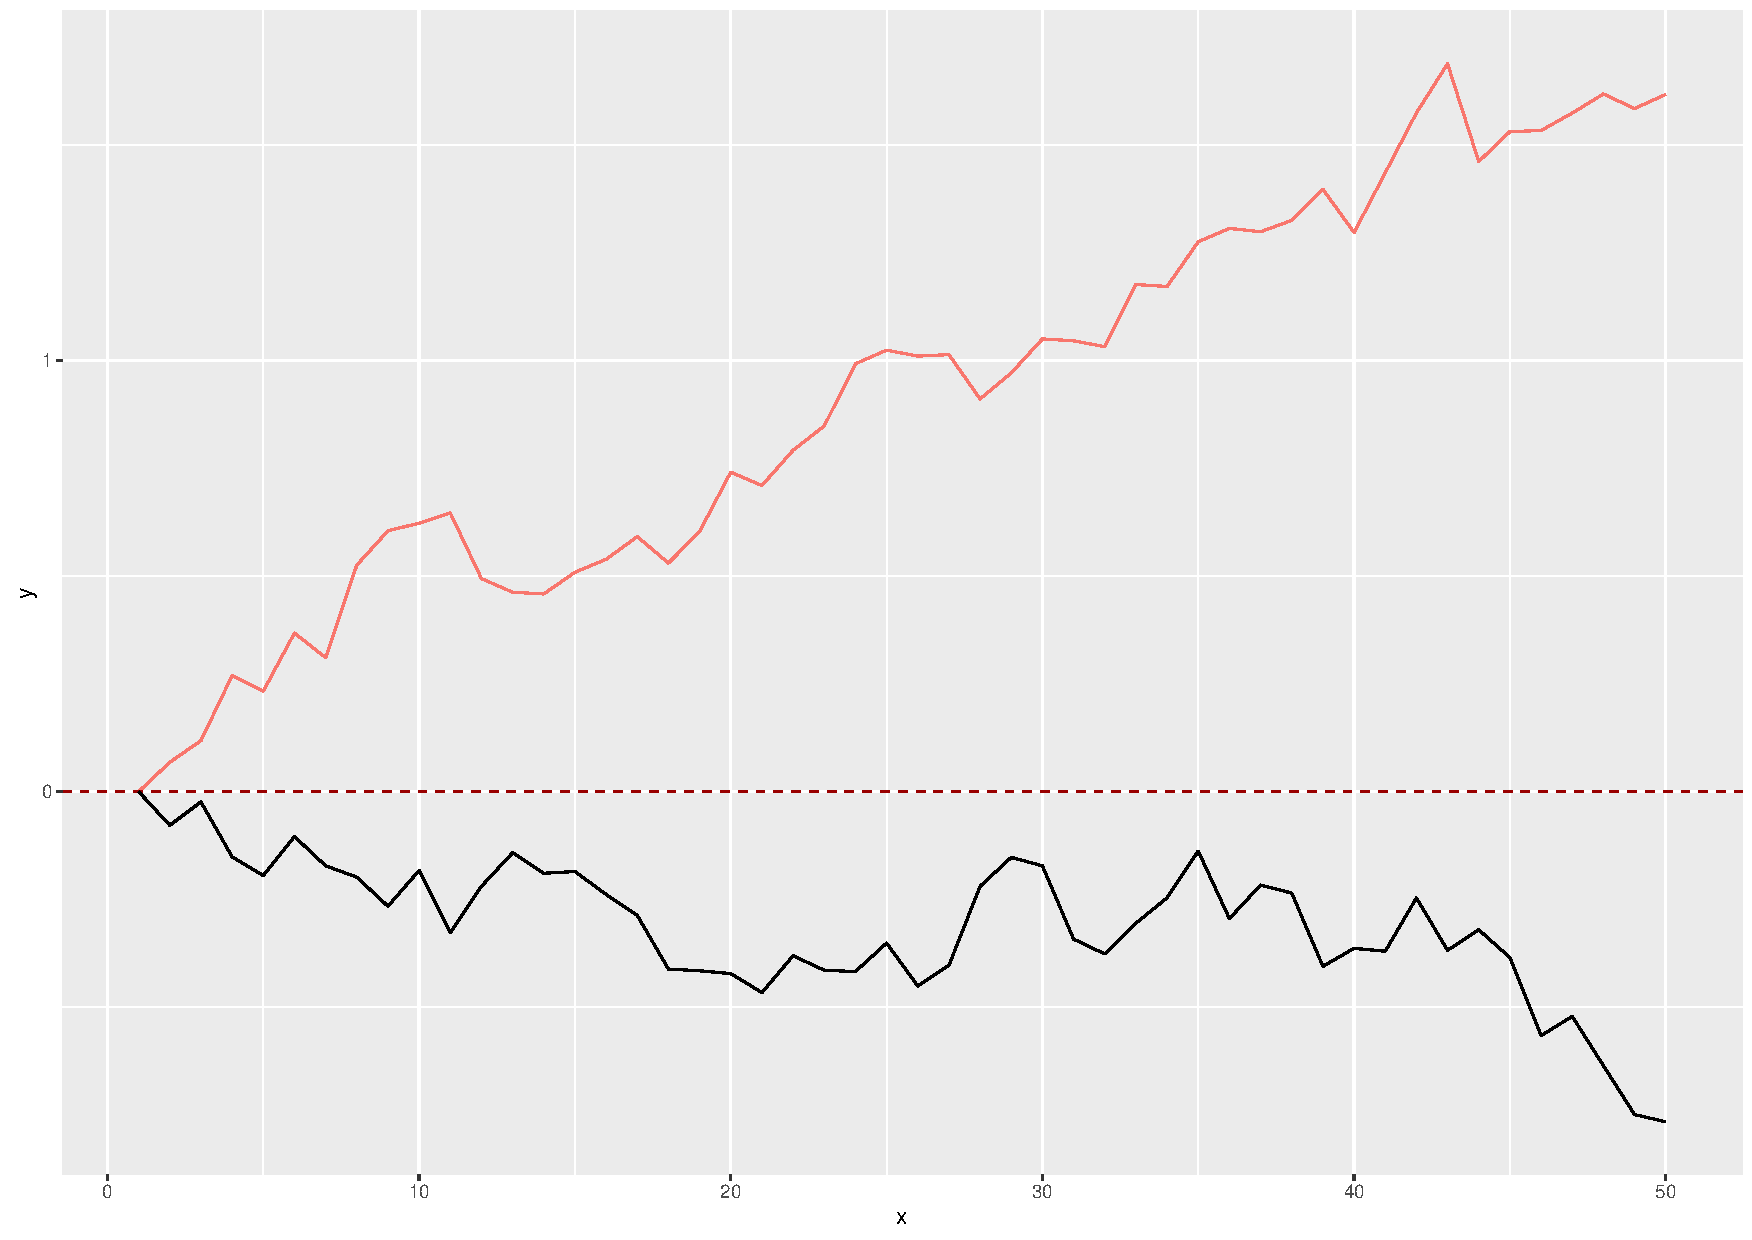
\includegraphics[width=0.7\textwidth]{img/random_walk.pdf}
\end{itemize}
\end{frame}

%---------------------------------------------

\begin{frame}{Examples of stochastic processes}
\begin{itemize}
\item Random walk with a drift
$$ y_t=\alpha_0+y_{t-1}+e_t \Rightarrow y_t =\alpha_0 t + e_{t} + e_{t-1} +  \dots +e_1 + y_0$$
A linear trend with random walk around the trend. \\ It is neither covariance stationary nor weakly dependent.
\begin{align}\nonumber
E(y_t) & =\alpha_0 t +E(y_0)\\\nonumber
Var(y_t) & =\sigma^2_e t\\\nonumber
Corr(y_t,y_{t+h}) & =\sqrt[]{t/(t+h)}
\end{align} 
Correlation decreases very slowly and decline speed depends on $t$.
\end{itemize}
\end{frame}

%---------------------------------------------

\begin{frame}{Examples of stochastic processes}
\begin{itemize}
\item Realization of random walk with a drift \\ 
\vspace{0.2cm}
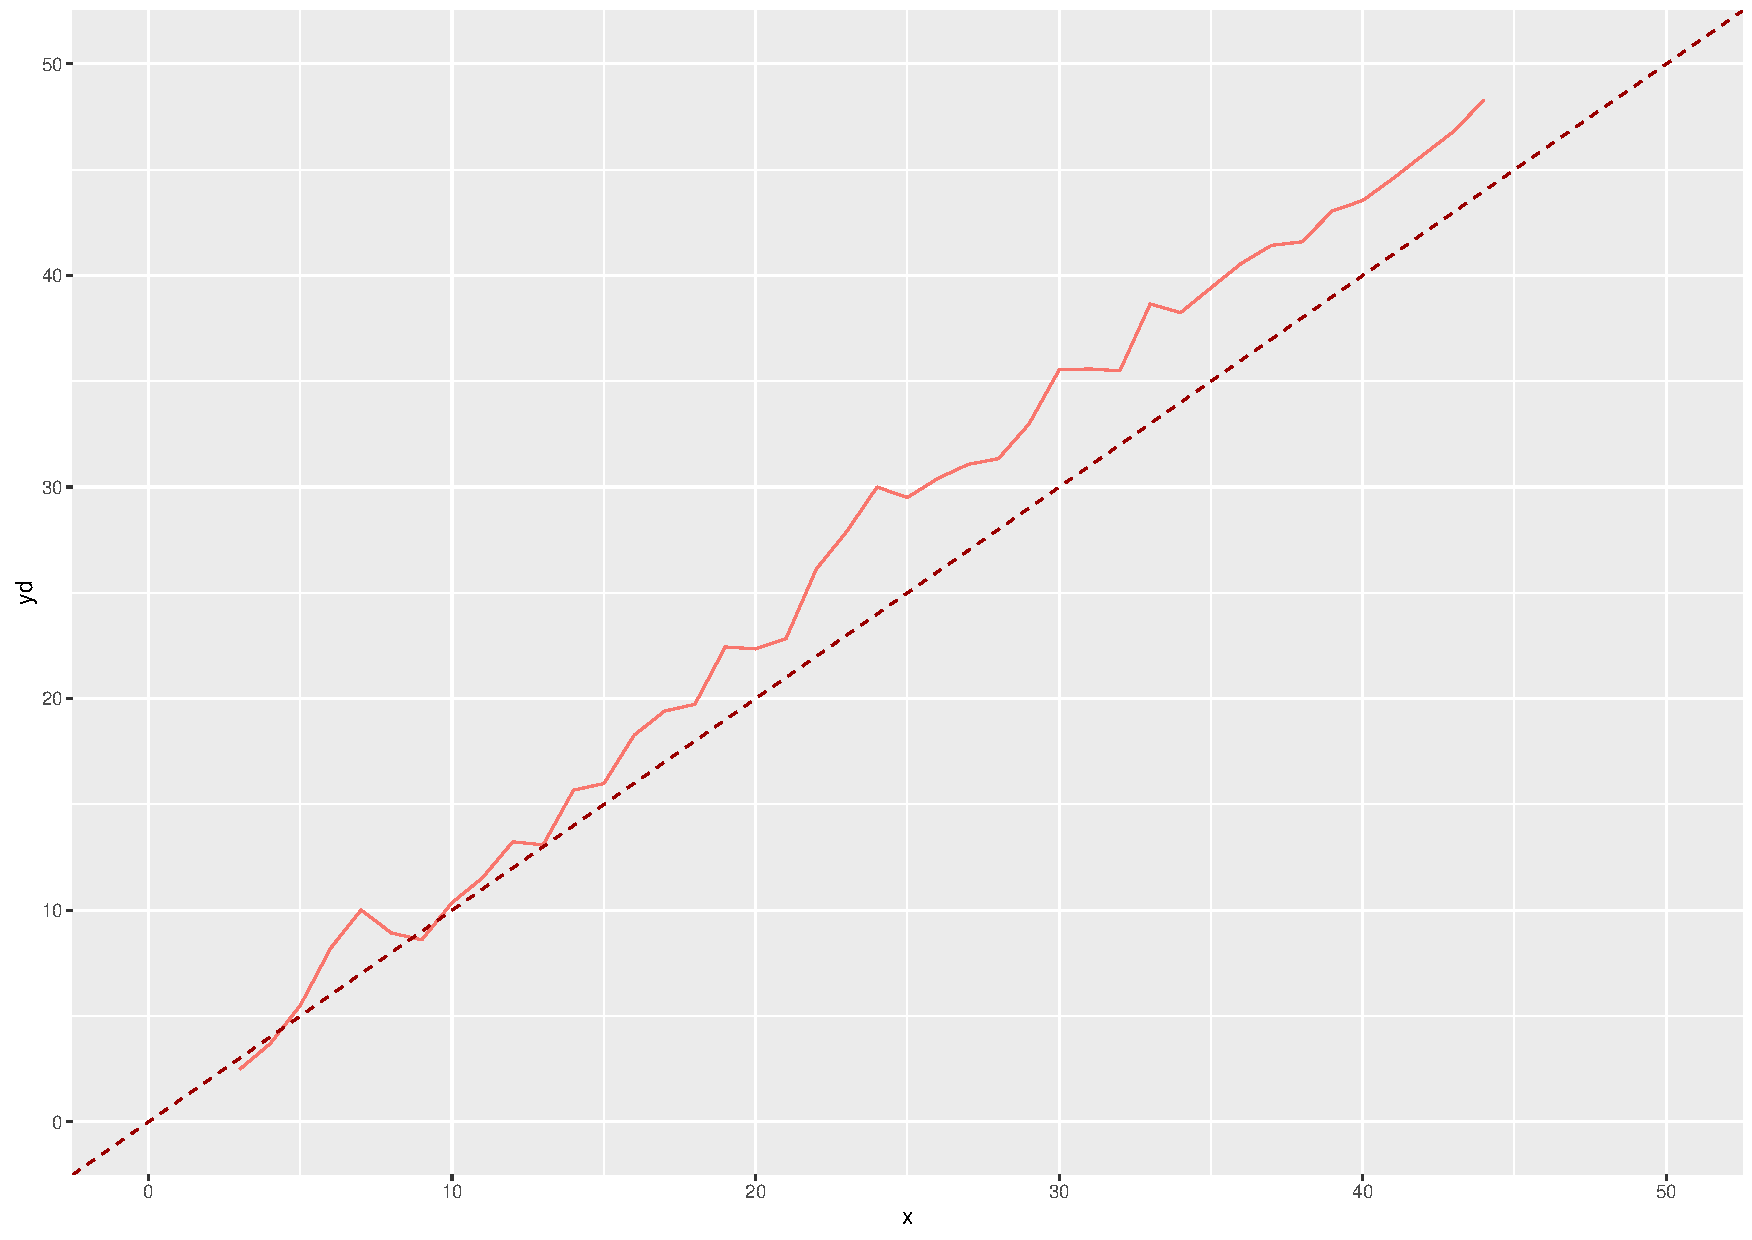
\includegraphics[width=0.7\textwidth]{img/random_walk_drift.pdf}

\item Different realizations of trending TS may produce \\similar time series.
\end{itemize}
\end{frame}

%---------------------------------------------
\section{Unit roots}
\begin{frame}{Examples of stochastic processes}

$y_t = \boxedd{$1 \cdot y_{t-1}$} + \boxedd{$u_t$} = y_{t-1} + u_t$
\medskip
\begin{itemize}
\item Unit root process: $y_t = y_{t-1} + u_t$; \quad  \\
$u_t$ is a weakly dependent series.
\item Random walk is a special case of the unit root process \\where: $u_t \sim \textit{Distr} \, (0, \sigma_u^2), \textit{iid}$
\bigskip
\end{itemize}

We need to distinguish strongly and weakly dependent TS:
%\vspace{0.5cm}
\begin{itemize}
\item Economic reasons: \\ In strongly dependent series, shocks or policy changes  have  long or permanent effects; in weakly dependent series, their effect  is only temporary.
\item Statistical reasons: \\ Analysis with strongly dependent series must be handled in specific ways.
\end{itemize}
\end{frame}

%---------------------------------------------

\begin{frame}{Integrated series}
\textbf{Terminology - Order of integration }
\vspace{0.5cm}
\begin{itemize}
\item Weakly dependent TS are integrated of order zero: $I(0)$.
\vspace{0.2cm}
\item If we have to difference a TS once to get a weakly dependent TS, then it is integrated of order 1: $I(1)$.
\vspace{0.2cm}
\item Example of a $I(1)$ process:
\begin{align}\nonumber
y_t & =y_{t-1}+e_t  \hspace{0.55cm} \Rightarrow \Delta y_t = y_t-y_{t-1}=e_t \\\nonumber
 \log{y_t} & =\log{y_{t-1}}+e_t  \Rightarrow \Delta \log{y_t}=e_t
 \end{align} 
 \item A time series is integrated of order $d$: $I(d)$, if it becomes \\a weakly dependent TS after being differenced $d$ times.
\end{itemize}
\end{frame}

%---------------------------------------------

\begin{frame}{Unit roots tests}
Unit root tests help to decide if a time series is $I(0)$ or not
\vspace{0.4cm}
\begin{itemize}
\item Use either some informal procedure or a unit root test
\vspace{0.4cm}
\item Informal procedures
\begin{itemize}
\item Analyze autocorrelation of the first order
$$\hat{\rho}_1=\hat{Corr}(y_t,y_{t-1})$$
\item If $\hat{\rho}_1$ approaches 1, it indicates that the series can have unit root. Alternatively, it could have a deterministic trend.
\end{itemize}
\item We can analyze sample autocorrelations using \\a correlogram
\end{itemize}
\end{frame}
%---------------------------------------------
\begin{frame}{Unit root tests}
Correlogram:  
$\, \, \, \, \rho_h = \frac{\textit{cov} \, (y_t, y_{t-h})}{\sigma_{y_t} \cdot \sigma_{y_{t-h}}}$

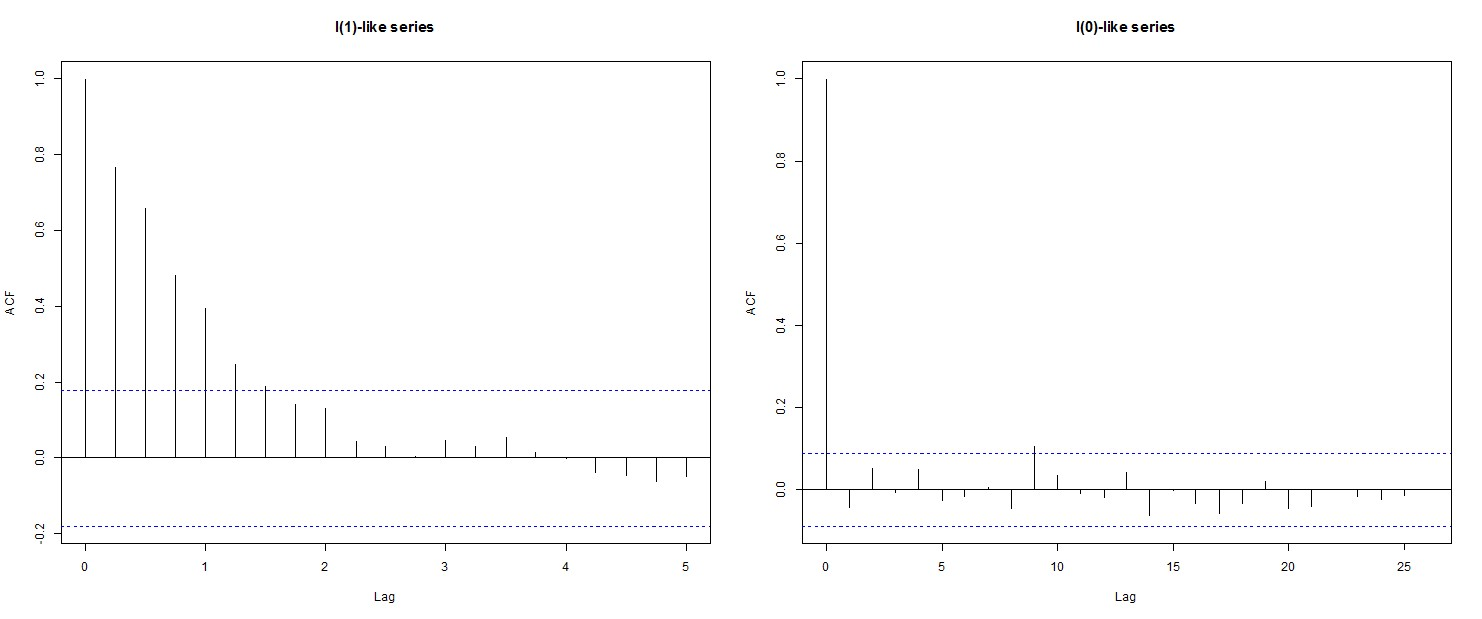
\includegraphics[width=1\textwidth]{img/corelogramWeek2.jpg}

\hspace{1.5cm} $I(1)$-like series \hspace{3 cm} $I(0)$-like series
\end{frame}
%---------------------------------------------
\begin{frame}{Unit root tests}
\textbf{Dickey-Fuller (DF) test} – motivation \\
\medskip
Unit root test in an $\textit{ar}(1)$ process: \\
\medskip
$y_t = \alpha + \rho y_{t-1} + e_t$\\
\medskip
$ H_0 : \rho = 1, \> \> \> H_1 : \rho <1$ \\
\medskip
\begin{itemize}
\item Under $H_0$, $y_t$ has a unit root. 
\begin{itemize}
\item[$\circ$] For  $\rho =1 \ \wedge \ \alpha =0 \rightarrow y_t$     is a random walk.
\item[$\circ$] For  $\rho =1 \ \wedge \ \alpha \neq 0 \rightarrow y_t$     is a randomw walk with a drift   \\and $E(y_t)$ is a linear function of $t$ .
\end{itemize}
\item Under $H_1$, $y_t$  is a weakly dependent $\textit{ar}(1)$ process. \\
\bigskip
\end{itemize}
\medskip
\end{frame}
%---------------------------------------------
\begin{frame}{Unit root tests}
\textbf{Dickey-Fuller (DF) test} – motivation \\
\medskip
Unit root test in an $\textit{ar}(1)$ process: \\
\medskip
$y_t = \alpha + \rho y_{t-1} + e_t$\\
\medskip
$ H_0 : \rho = 1, \> \> \> H_1 : \rho <1$ \\
\medskip
For DF tests, $H_1 : \rho <1$ is a common simplification to the full space of alternatives to $H_0: \rho = 1$.
\begin{itemize}
\item For $|\rho|<1$, $\,\, y_t$  is weakly dependent (as $\textit{plim} \> \rho^h=0$)\\
However, if unit root is likely to be present, the probability of $\rho<0$ is negligible.
\item We usually ignore the possibility of $\rho >1$   , as it would lead to explosive behavior in $y_t$. \\
\dots $|\rho|>1$ would allow for explosive oscillations in $y_t$.
\end{itemize}
\end{frame}
%---------------------------------------------
\begin{frame}{Dickey Fuller (DF) test}
\small
\begin{itemize}
\item Basic equation for unit root test in an $\textit{ar}(1)$ process: \qquad $ y_t = \alpha + \rho y_{t-1} + e_t $ \\
\item For DF test, we apply a suitable transformation to $y_t$:  \\we subtract $y_{t-1}$ from both sides of the equation:
\begin{flalign*}
& \Delta y_t  = \alpha + (\rho - 1) y_{t-1} + e_t; \text{ apply substitution: } \theta=(\rho-1)&&\\
& \text{i.e.} && \\
& \Delta y_t  = \alpha + \theta y_{t-1} + e_t;  \textrm{ now:} 
\end{flalign*}
\item We use a $t$-ratio for testing $H_0:\theta = 0. $   However:\\
Under $H_0$, $t$-ratios don't have a $t$-distribution, but follow a $DF$-distribution.  (-negative- critical values of the $DF$ distribution are much farther from zero)
\item Critical values for the $DF$ distribution are available from statistical tables and implemented in most relevant SW packages.
\end{itemize}
\begin{tikzpicture}[<-,overlay,remember picture,inner sep=1.5pt,shorten <=0.2em,font=\small]
\tikzset{
    mynode/.style={rectangle, minimum size=3cm, text width=6cm}
}
\node[mynode] at (9,4.2)(box){$H_0 \  : \rho = 1 \Leftrightarrow H_0 : \theta = 0$ \\
$H_1 \ : \rho < 1 \Leftrightarrow H_1 : \theta < 0$};
\tikzset{
    mynode/.style={rectangle, dashed, very thick, draw=Red, minimum size=0.9cm, text width=1.6cm}
}
\node[mynode] at (9,4.2) (A){};
\end{tikzpicture}
\end{frame}
%---------------------------------------------
\begin{frame}{DF test \& ADF test}
\footnotesize
Unit root time series can manifest various levels of complexity. Hence, DF  test is usually performed using the following three specifications: \\
\begin{minipage}[c]{.1\textwidth}
\begin{flalign*}
\Delta y_t  = \quad  & \theta y_{t-1} + e_t &&  \\
\Delta y_t  = \alpha \ + \ & \theta y_{t-1} + e_t && \\
\Delta y_t  = \alpha \ + \ & \theta y_{t-1} + \delta t + e_t && \\
\end{flalign*}
\end{minipage}
%
\begin{minipage}[c]{.5\textwidth}
random walk \\
random walk with a drift\\
random walk with a drift and trend
\end{minipage}
% 
\\
DF test is the same ($H_0: \theta = 0$) for all specifications   /critical values difffer/ \\
\medskip
\underline{Augmented Dickey-Fuller (ADF) test} is a common generalization of DF test\\
(example: Augmentation of the DF test for the $2^{nd}$ specification) 
$$\Delta y_t = \alpha + \rbox{$\theta y_{t-1}$} + \gamma_1 \Delta y_{t-1} + \dots + \gamma_p \Delta y_{t-p} + e_t$$
\begin{itemize}
\item When estimating $\theta$, we control for possible $\textit{ar}(p)$ behavior in $\Delta y_t$. 
\item ADF test has the same null hypothesis as a DF test $\rightarrow$ $H_0: \theta = 0$.
\end{itemize}
\begin{tikzpicture}[<-,overlay,remember picture,inner sep=1.5pt,shorten <=0.2em,font=\small]
\tikzset{
     mynode/.style={rectangle, dashed, very thick, draw=Red, minimum height=1.5cm, text width=0.8cm}
}
\node[mynode] at (2,5.5)(box){};
\end{tikzpicture}
\end{frame}
%---------------------------------------------

\begin{frame}{Unit root tests in R: package \{urca\}}
Description of the options for the \texttt{ur.df()} function:
\medskip
\begin{enumerate}
\item \texttt{type "none"} \\
$\Delta y_t = \theta y_{t-1} + e_t$ ~\\
\texttt{tau1:} we test for $H_0: \theta = 0$ (unit root) 
\medskip
\item \texttt{type "drift"} \\
$\Delta y_t = \alpha + \theta y_{t-1} + e_t$ ~\\
\texttt{tau2:} $H_0: \theta = 0$ (unit root) \\
\texttt{phi1:} $H_0: \theta = \alpha = 0$ (unit root and no drift) 

\medskip
\item \texttt{type "trend"} \\
$\Delta y_t = \alpha + \theta y_{t-1} + \delta t + e_t$ ~\\
\texttt{tau3:} $H_0: \theta = 0$ (unit root) \\
\texttt{phi2:} $H_0: \theta = \alpha = \delta = 0$ (unit root, no drift, no trend) 
\texttt{phi3:} $H_0: \theta = \delta = 0$ (unit root and no trend) 

\end{enumerate}
\end{frame}

%---------------------------------------------

\begin{frame}{Unit root tests}
\begin{itemize}
\item ADF test for TS with trend
$$ \Delta y_t = \alpha  + \theta y_{t-1} + \delta t + \gamma_1\Delta y_{t-1}+\dots+\gamma_p\Delta y_{t-p}+e_t$$
Under the alternative hypothesis of no unit root, the process is trend-stationary.
\medskip
\item The critical values in the ADF distribution with time trend are even more negative as compared to random walk and random walk with a drift.
\medskip
\item When using DF/ADF specification 1 or 2 (R-W, R-W with drift) to test for unit root in a clearly trending TS, the test would not have sufficient power (we would not reject $H_0$ for trending weakly dependent TS).
\end{itemize}
\end{frame}

%---------------------------------------------

\begin{frame}{Unit roots and trend-stationary series}
\begin{itemize}
\item $ \Delta y_t = \alpha  + \theta y_{t-1} + \delta t + \gamma_1\Delta y_{t-1}+\dots+\gamma_p\Delta y_{t-p}+e_t$
\vspace{0.2cm}
\item Terminology:
\vspace{0.2cm}
\begin{itemize}
\item Stochastic trend: $\theta=0$ \\
Also called \textbf{difference-stationary process}: $y_t$ can be turned into $I(0)$ series by differencing. Terminology emphasizes stationarity after differencing $y_t$ instead of weak dependence in differenced TS.
\vspace{0.2cm}
\item Deterministic trend: $\delta \neq 0, \hspace{0.3cm} \theta<0$ \\
Also called \textbf{trend-stationary process}: has a linear trend, not a unit root. $y_t$ is weakly dependent - $I(0)$ - around its trend. We can use such series in LRMs, if trend is also used as regressor.

\end{itemize}
\vspace{0.3cm}
\item DF/ADF tests are not precise tools. Distinguishing between stochastic and deterministic trend is not easy (sample size!). 
\end{itemize}
\end{frame}

%---------------------------------------------

\begin{frame}{Handling trend-stationary time series}
\begin{itemize}
\item Trend-stationary TS fulfill TS.1' assumption (look at Week1 presentation). \\ 
\vspace{0.5cm}
We can use them in regressions if we have time trend among regressors.
\end{itemize}
\end{frame}

%---------------------------------------------

\begin{frame}{Handling strongly dependent time series}
\begin{itemize}
\item Strongly dependent time series do not fulfill TS.1' assumption (look at Week1 presentation). We cannot use them in regressions directly.
\vspace{0.5cm}
\item Sometimes, taking logarithms helps.
\vspace{0.5cm}
\item Sometimes, we can transform such series into weakly dependent time series.
\vspace{0.5cm}
\item Differencing is popular, but it has drawbacks.
\end{itemize}
\end{frame}
%---------------------------------------------

\begin{frame}{Handling strongly dependent time series}
\begin{block}{Example}
\vspace{-0.5cm}
\begin{align} 
y_t & = \beta_0 + \beta_1 x_t + \varepsilon_t & y_t, x_t \sim I(1) \\
y_{t-1} & = \beta_0 + \beta_1 x_{t-1} + \varepsilon_{t-1} & \varepsilon_t \sim i.i.d. \\
\Delta y_t & = \qquad \, \beta_1\Delta x_t + v_t  & v_t= \varepsilon_t - \varepsilon_{t-1}
\end{align}
\end{block}
\begin{enumerate}
\item If we work with logarithms, it has an additional advantage: \\
$\log y_t - \log y_{t-1} = \log \left( \frac{y_t}{y_{t-1}} \right) \doteq\frac{y_t - y_{t-1}}{y_{t-1}}$ \\ 
i.e.: nice interpretation as rate of growth of $y_t$
\item Three problems 
\begin{enumerate}
\item $v_t$ is no more i.i.d.
\item We loose information linked with the levels of variables, short term relation are stressed
\item Estimates often generate bad long-term predictions: 
$ \Delta \hat{y}_t = \hat{\beta}_1 \Delta x_t$; $ \dots $ what if $\beta_0 \neq 0$? 
\end{enumerate}
\end{enumerate}
\end{frame}

%---------------------------------------------

\begin{frame}{Handling strongly dependent time series}

Some properties of integrated processes
\vspace{0.5cm}
\begin{enumerate}
\item The sum of stationary and non-stationary series must be non-stationary.
\item Consider a process $y_t=\alpha + \beta x_t$:\\
~$\cdot$~~ If $x_t$ is stationary then $y_t$ will be stationary. \\
~$\cdot$~~ If $x_t$ is non-stationary then $y_t$ will be non-stationary. 
\item If two time series are integrated of different orders, then any linear combination of the series will be integrated at the higher of the two orders of integration. 
\item Sometimes it turns out a linear combination of two $I(d)$ series is integrated of order less then $d$. 
\end{enumerate}
\end{frame}

%---------------------------------------------
\section{Cointegration}

\begin{frame}{Spurious regression or cointegration}
\begin{itemize}
\item \textbf{Spurious regression}
 Regressing one $I(1)$-series on another $I(1)$-series may lead to extremely
high $t$-statistics even if the series are completely independent. Similarly, the $R^2$ of such regressions tend to be very high. \\Regression analysis involving time series that have a unit root may generate completely misleading inferences.
\vspace{0.5cm}
\item \textbf{Cointegration} Fortunately, regressions with $I(1)$-variables are not always spurious:
If there is a stable relationship between time series that, individually, display unit root behavior, these time series are called ``cointegrated''.
\end{itemize}
\end{frame}

%---------------------------------------------

\begin{frame}{Spurious regression or cointegration}
\textbf{General definition of cointegration}\\
\vspace{0.5cm}
Two $I(1)$-time series $y_t$, $x_t$ are said to be cointegrated if there exists a stable relationship between them, where:
$$ y_t=\alpha+\beta x_t + e_t, 
\hspace{0.5cm} e_t \sim I(0)$$
\textbf{Cointegration (CI) test if CI parameters are known}\\
\vspace{0.5cm}
For residuals of the known CI relationship:
$$e_t := y_t-\alpha-\beta x_t, $$
test whether the residuals have a unit root (DF/ADF and other unit root tests may be applied ``directly''). \\If the unit root $H_0$ is rejected, $y_t$, $x_t$ are cointegrated. 
\end{frame}

%---------------------------------------------

\begin{frame}{Spurious regression or cointegration}
\begin{itemize}
\item \textbf{Testing for CI if the parameters are unknown}\\
If the potential relationship is unknown, it can be estimated by OLS. After that, we test whether the regression residuals have a unit root. If the unit root is rejected, this means that $y_t$, $x_t$ are cointegrated. Due to the pre-estimation of parameters, critical values are different than in the case of known parameters. \\(Software handles this automatically.)
\item \textbf{The CI relationship may include a time trend}\\
If the two series have differential time trends (drifts in this case), the deviation between them may still be $I(0)$ but with a linear time trend. In this case one should include a time trend in the CI-regression. Also, we have to use different critical values when testing residuals.
\\(Software handles this automatically.)
\end{itemize}
\end{frame}

%---------------------------------------------

\begin{frame}{Cointegration tests based on regression residuals}
\textbf{Engle-Granger test} estimates a $p$-lag ADF equation:\\
$$
\Delta \hat{u}_t = \theta \, \hat{u}_{t-1} +
\sum_{j=1}^p \Delta \hat{u}_{t-j} + e_t
$$
\begin{itemize}
    \item Esentially, this is an ADF test on $\hat{u}_t$ [$\theta = (\rho -1)$]
    \item Specific critical values apply (farther from 0 than $t$ or $DF$).\\~\\
\end{itemize}

\textbf{Phillips-Ouliaris test} estimates a DF equation:\\
\vspace{-0.3cm}
$$\Delta \hat{u}_t = \theta \, \hat{u}_{t-1} + e_t$$
\vspace{-0.5cm}
\begin{itemize}
    \item The $t$-ratio is based on robust standard errors,\\different estimators exist for the robust standard errors.
\end{itemize}
\medskip
In both cases (EG and PO), $H_0$ of unit root in $\hat{u}$ \\i.e. ``no-cointegration'' is tested.
\end{frame}

%---------------------------------------------

\section{Error correction models}
\begin{frame}{Error correction model (ECM)}
\begin{itemize}
\item It can be shown that when variables are cointegrated, i.e. when there exists a long-term relationship among them, their short-term dynamics are related as in a so-called error correction model (ECM).
\end{itemize}
\end{frame}

%---------------------------------------------

\begin{frame}{Error Correction Models - motivation}

\textbf{Autoregressive distributed lag models}\\
\medskip
\begin{itemize}
\item Autoregressive distributed lag model with one regressor
$$\textnormal{ADL}(p,q)\!: \, y_t = \beta_0 \, + \sum_{i=1}^p \beta_i y_{t-i} \, + 
         \sum_{j=0}^q \gamma_j x_{t-j} + u_t, \hspace{0.2cm}
         u_t \sim iid(0,\sigma^2)$$

\item There are many useful modifications/simplifications to the $\textnormal{ADL}(p,q)$ process. For example:
\begin{equation} \label{ADL11}
\textnormal{ADL}(1,1)\!: \, y_t = \beta_0 + \beta_1 y_{t-1} + 
         \gamma_0 x_t + \gamma_1 x_{t-1} + u_t \,.
\end{equation}
%~\\         
Additional ADL$(1,1)$ restriction: $\beta_1 = 1$ and $\gamma_1 = -\gamma_0$
$$\textnormal{gives a model in $1^{st}$ diffs.: } \,\,\, \Delta y_t = \beta_0 + \gamma_0 \Delta x_t + u_t\,. $$
\end{itemize}

\end{frame}

%---------------------------------------------
\begin{frame}{Error Correction Models - motivation}

For ADL(1,1) model \eqref{ADL11}, suppose there is an equilibrium value $x^{\circ}$ and in the absence of shocks, $x_t \rightarrow x^{\circ}$ as $t \rightarrow \infty$. Then, assuming absence of $u_t$ errors, $y_t$ converges to steady state: $y^{\circ}$.\\ 
\medskip
Hence, the ADL(1,1) model \eqref{ADL11} can be re-written as:
$$y^{\circ} = \beta_0 + \beta_1 y^{\circ} + (\gamma_0 + \gamma_1) x^{\circ}$$

Solving this for $y^{\circ}$ as a function of $x^{\circ}$, we get

$$ y^{\circ} = 
   \frac{\beta_0}{1 - \beta_1} + \frac{\gamma_0 + \gamma_1}{1 - \beta_1} x^{\circ} = 
   \frac{\beta_0}{1 - \beta_1} + \lambda x^{\circ}$$
where $ \lambda \equiv \frac{\gamma_0 + \gamma_1}{1 - \beta_1}$ and $|\beta_1|<1$ is assumed. \\


\end{frame}
%---------------------------------------------
\begin{frame}{Error Correction Models - motivation}

$$ y^{\circ} =  \frac{\beta_0}{1 - \beta_1} + \lambda x^{\circ}$$

$$ \lambda \equiv \frac{\gamma_0 + \gamma_1}{1 - \beta_1}$$

\begin{itemize}
\item $\lambda$ is the long-run derivative of $y^{\circ}$ with respect to $x^{\circ}$.
\medskip
\item $\lambda$ is an elasticity if both $y^{\circ}$ and $x^{\circ}$ are in logs.
\medskip
\item $\hat{\lambda}$ can be computed directly from the estimated parameters of the ADL(1,1) model \eqref{ADL11}.
\end{itemize}


\end{frame}
%---------------------------------------------
\begin{frame}{Error Correction Models - motivation}

The ADL(1,1) equation \eqref{ADL11} - repeated here for convenience:
\begin{equation*}
y_t = \beta_0 + \beta_1 y_{t-1} + 
         \gamma_0 x_t + \gamma_1 x_{t-1} + u_t,
\end{equation*}
can be equivalently rewritten as follows:
\begin{equation} \label{ECM}
\Delta y_t = \beta_0 + (\beta_1 -1) ( y_{t-1} - \lambda x_{t-1} ) + 
         \gamma_0 \Delta x_t + u_t.
\end{equation}
Again, $ \lambda \equiv \frac{\gamma_0 + \gamma_1}{1 - \beta_1}$ and $|\beta_1| < 1$ is assumed. \\
\medskip
Equation \eqref{ECM} is an error-correction model (ECM).
\end{frame}
%---------------------------------------------
\begin{frame}{Error Correction Models}
\begin{equation*} 
\textnormal{ECM:} \, \, \, \Delta y_t = \beta_0 + (\beta_1 -1) ( y_{t-1} - \lambda x_{t-1} ) + 
         \gamma_0 \Delta x_t + u_t.
\end{equation*}

\begin{itemize}
\item $( y_{t-1} - \lambda x_{t-1} )$ measures the extent to which the long run equilibrium between $y_t$ and $x_t$ is not satisfied (at $t-1$).
\item Consequently, $(\beta_1 -1)$ can be interpreted as the proportion of the disequilibrium $( y_{t-1} - \lambda x_{t-1} )$ that is reflected in the movement of $y_t$, i.e. in $\Delta y_t$.
\item $(\beta_1 -1)( y_{t-1} - \lambda x_{t-1} )$ is the \textbf{error-correction term}.
\item Many ADL$(p,q)$ specifications can be re-written as ECMs.
\item \textbf{ECMs can be used with non stationary TS} (Week 3).
\item ECMs $(\beta_1 -1)$ is essentially the same as $\theta$ from \\Partial adjustment model (see Week 4).
\end{itemize}


\end{frame}
%---------------------------------------------
\begin{frame}
\begin{block}{Box 1: Partial Adjustment Models \\ {\small (Will be put into context in the 4th week)}}
\small
\begin{align}\label{eq:5}
Y_t^{\ast} = \alpha + \beta X_t + u_t  \hspace*{10mm} \parbox[t][2cm][t]{5cm}{Y_t^{\ast}: \textnormal{optimal or target value} \\ \textnormal{or long-run equilibrium value}}
\end{align}
\vspace*{-1.5cm} 
\begin{align}\label{eq:6}
Y_t - Y_{t-1} = \theta (Y_t^{\ast} - Y_{t-1})  \hspace*{4mm} \parbox[t][2cm][t]{5cm}{0 < \theta < 1 \\ \theta \,\, \sim \textnormal{coefficient of adjustment} \\ Y_t = \theta Y_t^{\ast} + (1-\theta) Y_{t-1}}
\end{align}
\vspace*{-1.2cm} 
\\\hspace*{5.1mm}As $\theta \rightarrow 1$, the speed of contemporaneous adjustment \\ \hspace*{5.1mm}of $Y_t$ towards $Y_t^{\ast}$ grows. \\
\vspace*{.5cm} 
\hspace*{5.1mm}Substituting $Y_t^{\ast}$ from \eqref{eq:5} to \eqref{eq:6} yields
\begin{align}\label{eq:7}
Y_t = \alpha \theta + \beta \theta X_t + (1-\theta) Y_{t-1} + \theta u_t
\end{align}
We estimate \eqref{eq:7} and then calculate parameters in \eqref{eq:5} and \eqref{eq:6}.
\end{block}
\end{frame}

%---------------------------------------------

\begin{frame}{Error Correction Models}
\underline{Some more complicated ECMs:}\\
\bigskip
\begin{itemize}
\item[1)] We can use higher order lags, e.g. ADL(2,2):
$$y_t = \beta_0 + \beta_1 y_{t-1} + \beta_2 y_{t-2} +
         \gamma_0 x_t + \gamma_1 x_{t-1} + \gamma_2 x_{t-2} + u_t,$$
to establish ECMs. It is again possible to rearrange and re-parametrize ADL(2,2) to get an ECM. More than one re-parameterization is possible.\\
\bigskip
\item[2)] More than two variables can enter into an equilibrium relationship. 
\end{itemize}
\end{frame}

%---------------------------------------------
\end{document}